\begin{center}
	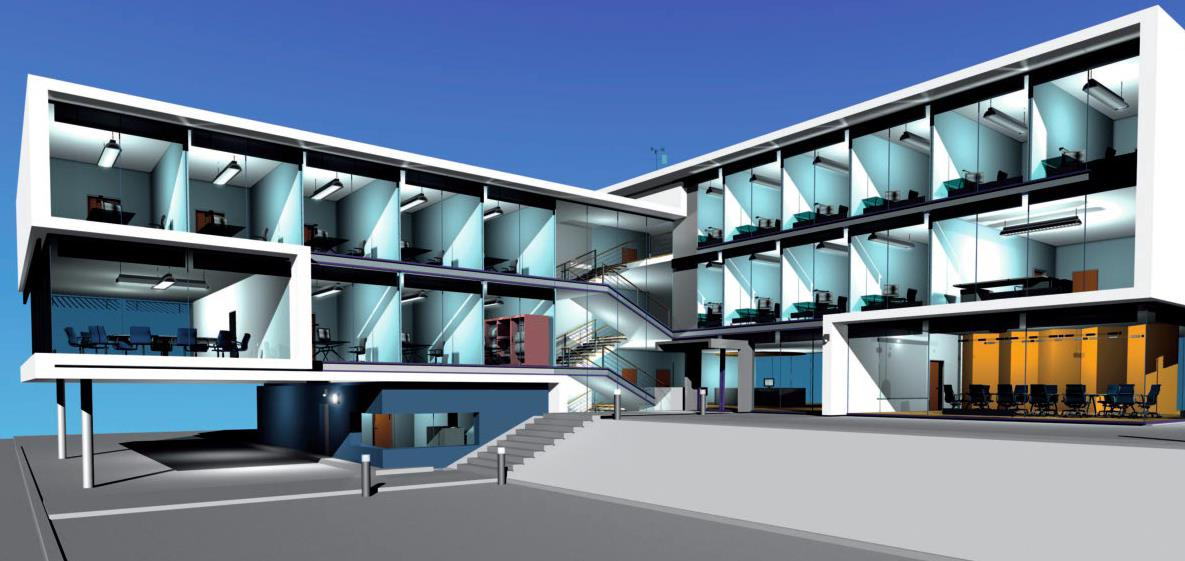
\includegraphics[width=0.75\linewidth]{illustrationBatiment.png}
\end{center}
\section{Introduction}

\subsection{Définition}
La Gestion Technique des Bâtiments (GTB) est un système permettant de contrôler, de surveiller et de réguler les équipements des bâtiments.
Ces équipements techniques sont notamment le chauffage, la climatisation, l'éclairage, les stores, la gestion d'accès et tout type d'alarmes liées à la sécurité ou à la maintenance du bâtiment.

\UPSTIobjectifs{
	\begin{multicols}{2}
		\begin{itemize}
			\item Assurer le confort et la sécurité des occupants
			\item Faciliter la maintenance des équipements
			\item Réduire les consommations d'énergie
			\item Fiabiliser et surveiller les installations
		\end{itemize}
	\end{multicols}
}
Ces objectifs sont atteints par l'interconnexion des équipements techniques et par la mise en place d'une supervision centralisée. Ce cours portera sur l'étude de la GTB et de certains de ses protocoles de communication.

\UPSTIinfo[Domotique ou GTB ?]{
	La domotique et la GTB sont deux domaines de la \textbf{Gestion Technique}. Celle-ci comprend notamment :
	\begin{description}
		\item[La domotique] pour la gestion automatisée des équipements d'une habitation particulière.
		\item[La Gestion Technique Centralisée] pour la gestion des équipements d'un seul domaine provenant d'un même site.
		\item[La Gestion Technique des Bâtiments] pour la gestion automatisée des équipements de plusieurs domaines techniques et de sécurité provenant d'un ou plusieurs bâtiments.
		\item[La télégestion] est la gestion à distance d'une installation.
	\end{description}

	La GTB s'apparente à la domotique, à plus grande échelle et avec des fonctionnalités plus poussées.
}


\subsection{Les domaines d'intervention d'une GTB}
\begin{center}
	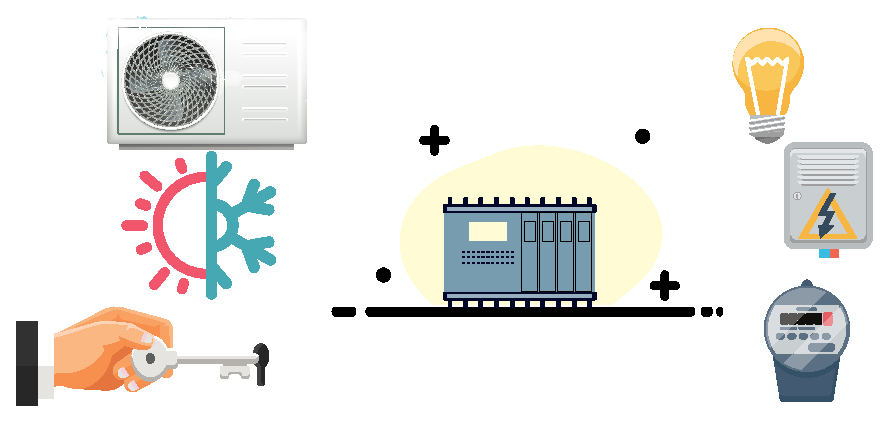
\includegraphics[width=0.75\linewidth]{domainesGTB}
\end{center}
\subsubsection{
\includegraphics[height=\iconeHeight]{chaudFroid} Le chauffage et la production de froid}
La GTB permet d'optimiser les temps de fonctionnement des chaudières et de réguler la température des locaux différemment selon l'occupation et l'utilisation de chaque zone. L'objectif visé étant de maximiser le confort des occupants tout en minimisant les consommations d'énergie.

Elle y parvient notamment par :
\begin{itemize}
	\item Le pilotage des chaudières : gestion, exploitation, suivi de consommation,
	\item La gestion des circuits de chauffage (circulateurs, vannes, etc.),
	\item La gestion des Centrales de Traitement d'Air (CTA) et des Centrales de Traitement d'Eau Glacée (CTEG) pour la production de froid.
	\item Une surveillance des capteurs du bâtiment (température, ouverture de fenêtre, présence, etc.).
\end{itemize}

\subsubsection{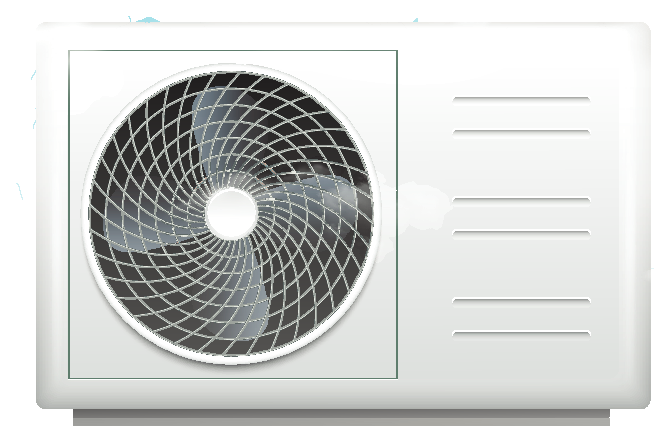
\includegraphics[height=\iconeHeight]{ventilation} La ventilation}
La GTB régule la ventilation en fonction de l'occupation des locaux et de la qualité de l'air. Elle gère également les débits d'air neuf et de reprise, contrôle les débits d'air et surveille les filtres. Cela optimise la consommation d'énergie en assurant une bonne qualité de l'air.

Elle y parvient par la gestion de la Centrale de Traitement d'Air (CTA).

\subsubsection{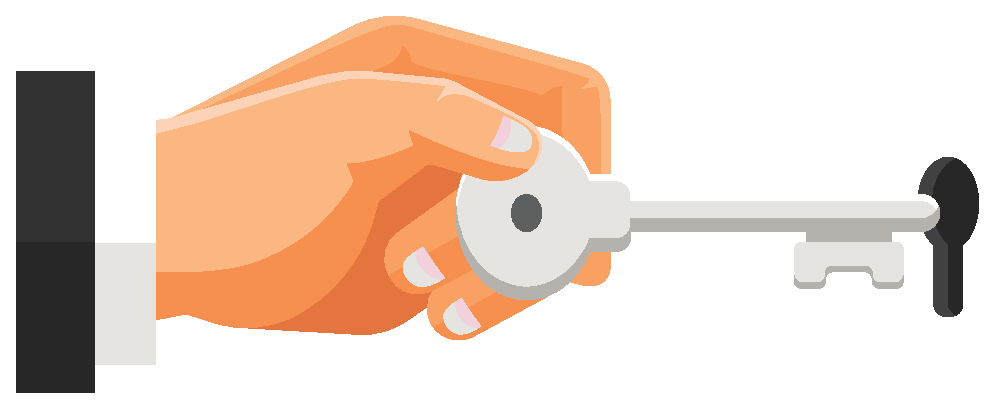
\includegraphics[height=\iconeHeight]{acces} La gestion d'accès}
La GTB gère les accès aux locaux en fonction des droits d'accès des occupants. Elle prévient les tentatives d'intrusions. Cette gestion se fait à l'aide de badges sécurisés, de reconnaissance vocale ou biométrique ainsi qu'à l'aide de capteurs de présence et d'intrusions.

\subsubsection{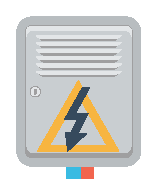
\includegraphics[height=\iconeHeight]{electricite} La gestion électrique}
La GTB pilote les éclairages, les convecteurs électriques, stores et volets roulants. Elle permet de réduire les consommations d'énergie en fonction de l'occupation des locaux et de la luminosité extérieure. Elle a la possibilité de délester automatiquement certains équipements afin de respecter un profil de consommation d'énergie.

Les compteurs électriques, comme les autres, sont scrutés par la GTB pour simplifier leur relevé et surveiller les consommations.

\subsection{Architecture matérielle d'une GTB}

\begin{UPSTIactivite}[][Architecture d'une GTB]
	\UPSTIeleveOnly{\vspace{6cm}}
	\UPSTIprofOnly{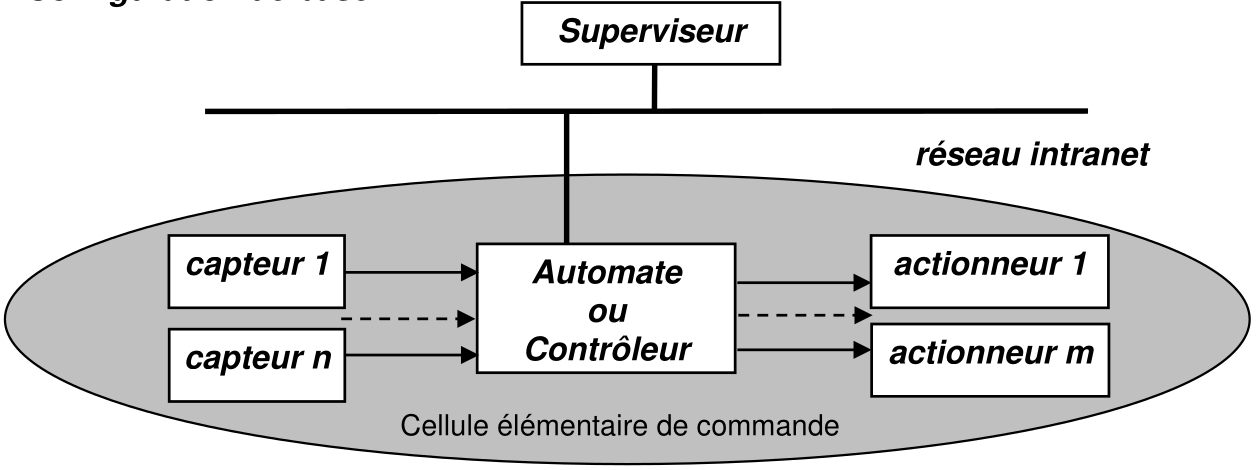
\includegraphics[height=5.5cm]{architectureGeneraleGTB}}
\end{UPSTIactivite}

\subsubsection*{Les capteurs}
Les capteurs permettent de connaître l'état du bâtiment. Ils relèvent par exemple :
\begin{multicols}{3}
	\begin{itemize}
		\item Température,
		\item Humidité,
		\item Pression,
		\item Luminosité,
		\item Présence,
		\item Ouverture de porte,
		\item Ouverture de fenêtre,
		\item Quantité de CO2,
		\item Ensoleillement,
		\item Consommation,
		\item Fumées
		\item etc.
	\end{itemize}
\end{multicols}

\subsubsection*{Les automates programmables}
Les différents automates programmables (\textbf{contrôleur}) reçoivent des informations sur l'état du bâtiment à partir des différents capteurs. A partir du comportement programmé, ils envoient des ordres aux actionneurs pour agir sur le bâtiment.

\subsubsection*{Les préactionneurs et actionneurs}
Les actionneurs agissent sur le bâtiment sur ordre de la GTB. Cela va du simple relais à la vanne motorisé, en passant par les moteurs de volet roulant, ballast électroniques, etc. 

\subsubsection*{Le superviseur}
Le superviseur permet de configurer et paramétrer l'installation, de proposer une interface à l'utilisateur résumant l'état de l'installation et d'effectuer un suivi des données (consommations, températures, etc.).

\subsubsection*{Le réseau de communication}
Le réseau de communication permet de relier les différents éléments. Il peut être filaire ou non, de type bus ou non, propriétaire ou non.
Les protocoles de communication propres à la GTB sont, entre autres :
\begin{multicols}{4}
    \begin{itemize}
	\item KNX,
	\item Modbus,
	\item BACnet.
	\item LonWorks.
	\item M-Bus.
	\item DALI.
	\item EnOcean.
	\item ZigBee.
\end{itemize}
\end{multicols}
